\subsubsection{Definition}

A one-dimensional homogenous aquifer is chosen to simulate a soil column experiment conducted by Harter et al. \cite{HarWag:00}. In the experiment, a constant flow rate was established, 2.5 pore volumes NaCl - tap water solution and 2.5 pore volumes \emph{Cryptosporidium parvum} solution ($1\times10^5$ oocysts per mL) were injected respectively, the outflow was continuously collected. Fig.~\ref{ExperimentSchematic} shows the schematic discription of the experiment.

\begin{figure}[htbp!]
\centering
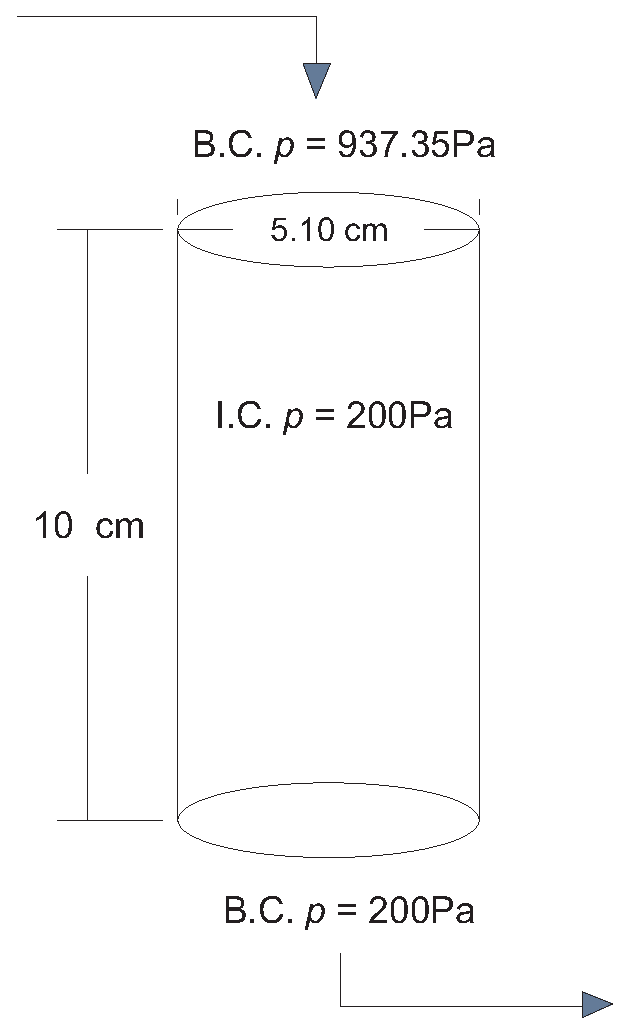
\includegraphics[scale=0.35]{PART_II/C/ExperimentSchematic.eps}
\caption{Soil column experiment}
\label{ExperimentSchematic}
\end{figure}

NaCl - tap water solution is used as tracer, which experiences only advection and dispersion. The \emph{Cryptosporidium parvum} can be classified as biological colloid. Colloids moving in porous media experience advection, dispersion, sorption-desorption, and filtration.

\subsubsection{Analytical solution}

For the one-dimensional transport including sorption-desorption and filtration through a homogeneous medium the following differential equation is applied

\begin{equation}\label{colloid transeq}
\frac{\partial C}{\partial t} + \frac{\rho_b}{n} \frac{\partial C_S}{\partial t} = v \alpha_L \frac{\partial^2 C}{\partial x^2} - v (\frac{\partial C}{\partial x} + \lambda C)
\end{equation}

where $C$ is dissolved concentration (kg$\cdot$m$^{-3}$), $C_S$ is sorbed concentration(kg$\cdot$kg$^{-1}$), $t$ is time (s), $\rho_b$ is bulk density (kg$\cdot$m$^{-3}$), $n$ is porosity (-), $v$ is velocity (m$\cdot$s$^{-1}$), $\alpha_L$ is longitudinal dispertivity (m), $x$ is distance (m), $\lambda$ is filtration coefficient (m$^{-1}$).

The instantaneous, linear sorption model assumes that
\begin{equation}\label{colloid sorption model}
C_S = K_{d} C
\end{equation}
where $K_{d}$ is the partitioning coefficient ($m^3 \cdot kg^{-1}$). The retardation coefficient $R$ is
\begin{equation}\label{colloid retardation coefficient}
R = 1 + \frac{\rho_b}{\theta} K_{d}
\end{equation}
The dispersion coefficient in $x$-direction $D_{xx}$ ($m^2 \cdot s^{-1}$) is
\begin{equation}\label{colloid dispersion x}
D_{xx} = v \alpha_L
\end{equation}
The analytical solution for a pulse input (inject time from 0 to $\tau$) is:
\begin{eqnarray}\label{colloid analytical 1}
C = & \frac{1}{2} C_0 &
\mbox{\hspace{-1.5ex}}\mbox{\hspace{-1.5ex}}
\left[
\exp
\left(
\frac{v x(1-\gamma)}{2 D_{xx}}
\right)
\mathrm{erfc}
\left(
\frac{x-v\gamma t/R}{2 \sqrt{D_{xx} t/R}}
\right)
\right. \nonumber\\[0.5ex]
& &
+\left.
\exp
\left(
\frac{v x(1+\gamma)}{2 D_{xx}}
\right)
\mathrm{erfc}
\left(
\frac{x+v\gamma t/R}{2 \sqrt{D_{xx} t/R}}
\right)
\right]
\end{eqnarray}
{\small
for $t \in (0, \tau) $ ,
}
\begin{eqnarray}\label{colloid analytical 2}
C = & \frac{1}{2} C_0 &
\mbox{\hspace{-1.5ex}} \mbox{\hspace{-1.5ex}}
\left[
\exp
\left(
\frac{v x(1-\gamma)}{2 D_{xx}}
\right)
\mathrm{erfc}
\left(
\frac{x-v \gamma t/R}{2 \sqrt{D_{xx} t/R}}
\right)
\right. \nonumber\\[0.5ex]
& &
+\left.
\exp
\left(
\frac{v x(1+\gamma)}{2 D_{xx}}
\right)
\mathrm{erfc}
\left(
\frac{x + v \gamma t/R}{2 \sqrt{D_{xx} t/R}}
\right)
\right. \nonumber\\[0.5ex]
& &
-\left.
\exp
\left(
\frac{v x(1-\gamma)}{2 D_{xx}}
\right)
\mathrm{erfc}
\left(
\frac{x - v\gamma (t - \tau)/R}{2 \sqrt{D_{xx} (t - \tau)/R}}
\right)
\right. \nonumber\\[0.5ex]
& &
-\left.
\exp
\left(
\frac{v x(1+\gamma)}{2 D_{xx}}
\right)
\mathrm{erfc}
\left(
\frac{x + v \gamma (t - \tau)/R}{2 \sqrt{D_{xx} (t - \tau)/R}}
\right)
\right]
\end{eqnarray}
{\small
for $t \in (\tau, \infty) $ , where
}
\begin{equation}\label{colloid analytical 3}
\gamma = \sqrt{1 + 4  v  \lambda  R  D_{xx} / v^2}
\end{equation}

\subsubsection{Numerical solution}

The calculation area is simplified to a line with the length of 0.1m. For the numerical model 100 elements and 101 nodes are included. Head gradient is set by giving two constant pressures at both left and right boundaries to establish a uniform velocity field with the value of 7.1 $md^{-1}$. 

The number of pore volume ($x$-axis) is calculated by

\begin{equation}\label{colloid pv}
P_{V} = \frac{v t}{L}
\end{equation}

where $v$ is the seepage velocity, $L$ is the length of the soil column. Considering the Courant number, the time step size is set by assigning $P_{V}$ to 0.01. In the simulation, 100 particles per time steps are loaded near the left boundary for 250 time steps.

The filtration process is described by using the filtration coefficient. The sorption-desorption process is described by the two-rate model from Johnson et al. \cite{JohBluLog:95}. In the two-rate model, desorption is governed by two different rate coefficients

\begin{equation}\label{colloid two-rate}
N/N_{0} = A e^{-k_{1}t} + (1-A) e^{-k_{2}t}
\end{equation}

where $N$ is the number of particles remaining on the medium at time $t$, $N_{0}$ is the initial number of particles on the medium at the time of initial sorption, $A$ is a weighting factor, $k_{1}$ and $k_{2}$ are the fast and slow sorption rate coefficient, respectively. Relative parameters are listed in Tab.~\ref{tab-colloid}.

\begin{table}[htbp!]
\caption{\label{tab-colloid}Model parameters for the column experiment}
\begin{center}
\begin{tabular}{llrr}
\toprule
Symbol & Parameter & Value & Unit \\
\midrule
$k$         & Permeability                    & $1.114476^{-11}$   & m$^{2}$ \\			
$\alpha _L$	& Longitudinal dispersivity       & 0.005              & m \\
$n$         & Porosity(tracer) 		            & 0.5                & $-$ \\
$n$         & Porosity(colloid)               & 0.42               & $-$ \\
$A$         & Weighting factor 		            & 0.9                & $-$ \\
$k_{1}$     & Fast sorption rate coefficient	& 0.1                & $-$ \\
$k_{2}$     & Slow sorption rate coefficient	& 0.001              & $-$ \\
$\lambda$   & Filtration coefficient        	& 5.2                & m$^{-1}$ \\
\bottomrule
\end{tabular}
\end{center}
\end{table}

\subsubsection{Results}

The tracer experiences only advection and dispersion, which means in Equation (\ref{colloid transeq}), $C_S = 0$, $\lambda = 0$. The results of RWPT simulation for the distribution of concentration over time are compared to those of measured value from the experiment by Harter, the analytical solution, and the OGS simulation with mass transport method. The comparison results are shown in Fig.~\ref{Tracertransport}.

\begin{figure}[htbp!]
\centering
\includegraphics[scale=0.35]{PART_II/C/Tracertransport.eps}
\caption{Tracer transport with advection and dispertion}
\label{Tracertransport}
\end{figure}

In the colloid transport simulation, the number of particles leaving the right boundary is counted each time step. The number is then converted to concentration in order to obtain the corresponding breakthrough curve over time. The comparison with the measured value from the experiment by Harter are shown in Fig.~\ref{ColloidTransport}.

\begin{figure}[htbp!]
\centering
\includegraphics[scale=0.4]{PART_II/C/ColloidTransport.eps}
\caption{Colloid transport with sorption-desorption and decay}
\label{ColloidTransport}
\end{figure}
